% RITMO - User Manual
%
% Built with XeLaTeX by build.sh (make-screenshots.sh makes the images from the program, md2tex.py
% the generated/*.tex fragments from the Markdown documents of doc/).
\documentclass[11pt,a4paper,oneside,openany]{book}

\usepackage[a4paper,margin=2.4cm,bottom=2.8cm]{geometry}
\usepackage{fontspec}
\setmainfont{Latin Modern Roman}
\setsansfont{Fira Sans}
\setmonofont{DejaVu Sans Mono}[Scale=MatchLowercase]
\usepackage{microtype}
\usepackage{xcolor}
\usepackage{graphicx}
\usepackage{float}
\usepackage{caption}
\usepackage{booktabs}
\usepackage{longtable}
\usepackage{array}
\usepackage{calc}
\usepackage{enumitem}
\usepackage{titlesec}
\usepackage{fancyhdr}
\usepackage{tcolorbox}
\usepackage{listings}
\usepackage[hidelinks]{hyperref}
\usepackage{bookmark}

% the colours of the logo
\definecolor{ritmoblue}{HTML}{0A0A28}
\definecolor{ritmoorange}{HTML}{FF6A2C}
\definecolor{ritmoyellow}{HTML}{FFD23C}
\definecolor{ritmomagenta}{HTML}{C63CC4}
\definecolor{ritmosky}{HTML}{3F8FD0}

\hypersetup{pdftitle={RITMO - User Manual},pdfauthor={RITMO contributors},
  pdfsubject={Atari POKEY music tracker},colorlinks=true,linkcolor=ritmosky!70!black,
  urlcolor=ritmosky!70!black}

\setlength{\parindent}{0pt}
\setlength{\parskip}{0.55em}
\setlist{itemsep=0.15em,topsep=0.3em}
\renewcommand{\arraystretch}{1.15}
\setlength{\emergencystretch}{3em}

% pandoc fragments
\providecommand{\tightlist}{\setlength{\itemsep}{0pt}\setlength{\parskip}{0pt}}
\newcommand{\passthrough}[1]{#1}

% chapter and section titles
\titleformat{\chapter}[display]
  {\sffamily\bfseries\color{ritmoblue}}{\large\color{ritmoorange}\MakeUppercase{\chaptertitlename}\ \thechapter}{0.3em}
  {\Huge}[\vspace{0.3em}{\color{ritmoorange}\titlerule[2pt]}]
\titleformat{\section}{\sffamily\Large\bfseries\color{ritmoblue}}{\thesection}{0.7em}{}
\titleformat{\subsection}{\sffamily\large\bfseries\color{ritmoblue}}{\thesubsection}{0.7em}{}
\titleformat{\subsubsection}{\sffamily\normalsize\bfseries\color{ritmoblue}}{\thesubsubsection}{0.7em}{}
\titlespacing*{\chapter}{0pt}{-10pt}{22pt}

\pagestyle{fancy}
\fancyhf{}
\fancyhead[L]{\sffamily\small\leftmark}
\fancyhead[R]{\sffamily\small RITMO}
\fancyfoot[C]{\sffamily\small\thepage}
\renewcommand{\headrulewidth}{0.3pt}
\fancypagestyle{plain}{\fancyhf{}\fancyfoot[C]{\sffamily\small\thepage}\renewcommand{\headrulewidth}{0pt}}

\captionsetup{font={small,sf},labelfont={bf,color=ritmoorange},labelsep=period}

% a screenshot: \shot{file}{caption}{width as a fraction of the text width}
\newcommand{\shot}[3]{%
  \begin{figure}[H]\centering
    \fbox{\includegraphics[width=#3\textwidth]{images/#1.png}}%
    \caption{#2}\label{fig:#1}%
  \end{figure}}
% a screenshot of a dialog, at its own size: \dialog{file}{caption}{width in cm}
\newcommand{\dialog}[3]{%
  \begin{figure}[H]\centering
    \fbox{\includegraphics[width=#3]{images/#1.png}}%
    \caption{#2}\label{fig:#1}%
  \end{figure}}

% names and keys
\newcommand{\key}[1]{\texttt{\small #1}}
\newcommand{\menu}[1]{\textsf{\textbf{#1}}}
\newcommand{\RITMO}{\textsf{RITMO}}
\newcommand{\RMT}{\textsf{RMT}}

\newtcolorbox{note}[1][Note]{colback=ritmoyellow!12,colframe=ritmoorange!80,fonttitle=\sffamily\bfseries,title=#1,
  boxrule=0.6pt,arc=2pt,left=6pt,right=6pt,top=4pt,bottom=4pt}
\newtcolorbox{tip}[1][Tip]{colback=ritmosky!8,colframe=ritmosky!80,fonttitle=\sffamily\bfseries,title=#1,
  boxrule=0.6pt,arc=2pt,left=6pt,right=6pt,top=4pt,bottom=4pt}

\lstset{basicstyle=\ttfamily\small,backgroundcolor=\color{black!4},frame=single,rulecolor=\color{black!20},
  breaklines=true,columns=fullflexible,keepspaces=true,xleftmargin=2pt,xrightmargin=2pt,
  literate={Š}{{\v{S}}}1}

\input{generated/version.tex}

\begin{document}

% ---------------------------------------------------------------- title page
\begin{titlepage}
  \centering
  \vspace*{1.2cm}
  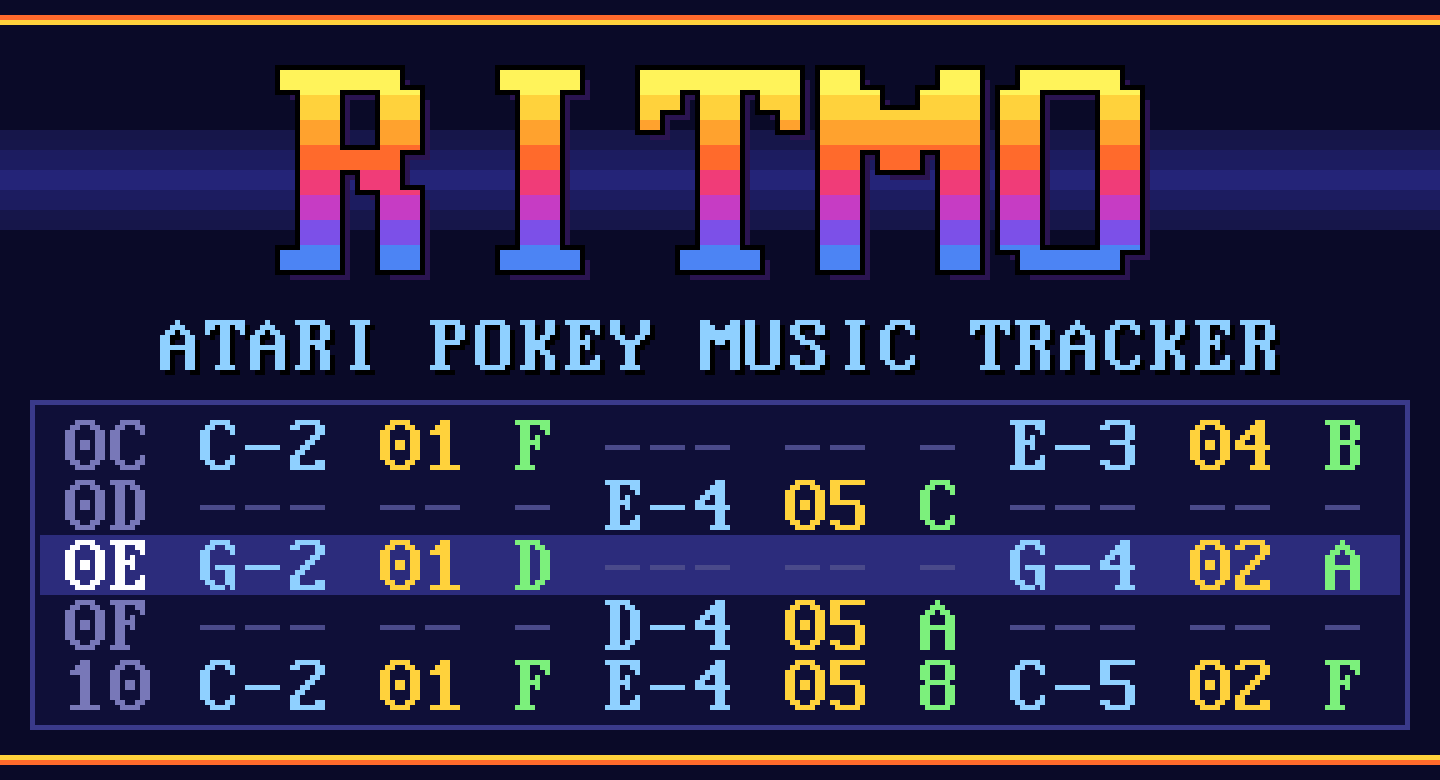
\includegraphics[width=\textwidth]{../logo/ritmo-logo.png}\par
  \vspace{1.4cm}
  {\sffamily\bfseries\fontsize{34}{40}\selectfont\color{ritmoblue} User Manual\par}
  \vspace{0.6cm}
  {\sffamily\Large Version \RitmoVersion\par}
  \vspace{2.2cm}
  {\sffamily\large
  A music tracker for the POKEY sound chip\\of the Atari 8-bit computers (XL/XE)\par}
  \vfill
  {\small Based on RASTER Music Tracker by Radek \v{S}t\v{e}rba (R.I.P.), VinsCool and Peter Dell (JAC!)\\[0.4em]
  \RitmoDate\par}
\end{titlepage}

\frontmatter
\chapter*{About this manual}
\addcontentsline{toc}{chapter}{About this manual}

This manual describes \RITMO{}, a music tracker for the POKEY sound chip of the Atari XL/XE
8-bit computers. \RITMO{} (\emph{\RITMO{} Is a Tracker for Music On Atari}) is a fork of the
RASTER Music Tracker (\RMT{}), and runs on Linux, Windows and macOS.

It is written for two kinds of reader: the musician who wants to compose, and the Atari
programmer who wants to use the result in a demo or a game. Chapters~\ref{ch:intro} to
\ref{ch:tutorial} introduce the program and walk through a first song; the next ones describe
every part of the window, the menus, the dialogs, the import and export formats, MIDI input
and the scripting; the appendices are the complete reference of the keys, the fields and the
file format.

\section*{Conventions}

\begin{itemize}
  \item Keys are written like \key{CONTROL+S} or \key{F5}. \key{CONTROL} is the \key{Ctrl} key
        (on macOS the \key{Control} key, not \key{Command}).
  \item A menu item is written \menu{File $\rightarrow$ Open\ldots}.
  \item Hexadecimal numbers have a \texttt{\$} in front: \texttt{\$3F} is 63. The tracker shows
        its numbers in hexadecimal: line numbers, instruments, volumes.
  \item The names of the fields of the screen are written as the program writes them, in capital
        letters: \texttt{VOLUME}, \texttt{TABLE LENGTH}.
  \item The screenshots are taken from the program itself, by the script
        \texttt{doc/manual/make-screenshots.sh}, with the default settings of a first start.
\end{itemize}

\begin{note}[RMT and RITMO in the reference]
The reference tables are converted from the documents of the original \RMT{}, and still call the program \RMT{} in places. \RMT{} is also the name of
the file format and of the player routines: an \emph{RMT module} and the \emph{RMT drivers} keep their names in \RITMO{}.
\end{note}

\begin{note}[Where the reference tables come from]
The tables of the menu commands, of the note keys, of the scripting commands and of the tracker
drivers (appendix~\ref{app:reference} and chapters~\ref{ch:drivers} and~\ref{ch:scripting}) are
converted from the Markdown documents in the \texttt{doc/} folder of the program, and the menu and note key
tables of those are written by the program itself (the \texttt{dump actions} and
\texttt{dump notekeys} script commands). They are always the state of the version this manual
is built from.
\end{note}

\tableofcontents

\mainmatter
\chapter{Introduction}\label{ch:intro}

\section{What \RITMO{} is}

The Atari XL/XE computers make their sound with the POKEY chip: four independent voices
(sixteen when two chips are used, as in many stereo songs), each with a frequency divider, a
choice of noise and tone distortions and a volume. A \emph{tracker} is the kind of music editor
that was born on the Amiga: the music is a grid of numbers, one column for each voice and one
row for each beat, and the notes are typed with the computer keyboard as on a piano.

\RITMO{} is such a tracker for the POKEY. A song made with it can be played on a real Atari: the
program produces the same data the player routines of the Atari read, and exports them in
several formats (a SAP file for the Atari players, an executable \texttt{.xex}, assembler source,
the compact RMT module for your own program). The sound you hear while composing comes from an
emulation of the Atari's 6502 processor and of the POKEY chip built into the program, running
the same player routine, so it is what the Atari will play.

\shot{window-tracks}{The main window of \RITMO{} with a song loaded.}{0.98}

\section{History}

\RITMO{} is a fork of the \emph{RASTER Music Tracker}, \RMT{}. The first version, 1.0, was
written by Radek \v{S}t\v{e}rba (Raster/C.P.U.) in 2002; his last version is 1.28, of 2009. It was
a small revolution for the Atari musicians: the first tracker for the POKEY with a
graphical envelope editor, and the one nearly everybody used. Radek \v{S}t\v{e}rba has since
passed away; this manual is, among other things, a way to remember his work. R.I.P.

Vin Samuel (\emph{VinsCool}) continued the program from 2021 to 2024, up to the version 1.34: a
new player routine with more tuning tables, a tuning calculator, an automatic high pass filter,
the SAP and XEX export and many corrections. Peter Dell (\emph{JAC!}) carries on the original
project from 2024 (version 1.35 and the planned version 2) and made it possible for this fork
to exist: everything described here is built on his work.

The \RITMO{} fork keeps the code of the tracker, the file formats and the player routines of
\RMT{} 1.35, and replaces what tied it to Windows. It is renamed so that it cannot be confused with the original
\RMT{}, and so that the Windows-only (MFC) parts of the code could be removed.

\section{What is different from \RMT{}}

\begin{itemize}
  \item The program is written with Qt: it runs natively on Linux, on Windows and on macOS (Intel and
        Apple Silicon). The look of the tracker screen is the original one, pixel for pixel.
  \item The 6502 and the POKEY emulations are built in: the \texttt{sa\_c6502.dll} and
        \texttt{apokeysnd.dll} libraries of the Windows versions are not needed any more.
  \item The sound goes out through PortAudio, and the MIDI input comes in through RtMidi.
  \item The configuration is kept per user in the settings of the system, not in an \texttt{.ini}
        file next to the program. The settings of \RMT{} are taken over at the first start.
  \item Songs, instruments and tracks are the same files as in \RMT{} 1.3x: you can move your work
        between the programs. The files keep their extensions, \texttt{.rmt} and the others.
\end{itemize}

\section{Files used by \RITMO{}}

\begin{center}
\begin{tabular}{@{}p{3.6cm}p{10.4cm}@{}}
\toprule
Extension & Content \\ \midrule
\texttt{.rmt} & an RMT module: the song, its tracks and its instruments (and, if the song was saved
                with \menu{Save}, the names of the song and of the instruments) \\
\texttt{.txt} & the same song as a text file, which can be read and edited with any editor; a single track is saved as a text file too \\
\texttt{.rmw} & a song work file: an RMT module with the state of the editing \\
\texttt{.rti} & a single instrument \\
\texttt{.sap}, \texttt{.sapr}, \texttt{.xex}, \texttt{.asm}, \texttt{.wav}, \texttt{.lzss} & the exported formats (chapter~\ref{ch:importexport}) \\
\texttt{.mod}, \texttt{.tmc}, \texttt{.tm8} & the formats that can be imported \\
\texttt{.rmtscript} & a script (chapter~\ref{ch:scripting}) \\
\bottomrule
\end{tabular}
\end{center}

\chapter{Installing and starting}\label{ch:install}

\section{The packages}

Everything the program needs is inside each package: the tracker drivers and the other files it
loads at run time are in the \texttt{resources} folder next to the program.

\begin{center}
\begin{tabular}{@{}>{\raggedright\arraybackslash}p{3.0cm}>{\raggedright\arraybackslash}p{4.6cm}>{\raggedright\arraybackslash}p{6.2cm}@{}}
\toprule
System & Package & How to start it \\ \midrule
Linux x86\_64 (Debian 11, Ubuntu 20.04 and newer) & \texttt{Ritmo-Linux-\allowbreak x86\_64.AppImage} &
  make it executable (\texttt{chmod +x}) and run it \\
Windows 64 bit & \texttt{Ritmo-Windows-x64-Setup.exe}, \texttt{Ritmo-Windows-x64.zip} &
  run the installer (it asks whether to install for all the users or for the current one, and offers a desktop icon and the
  \texttt{.rmt} file type), or unzip the archive anywhere and run \texttt{Ritmo.exe} (the program is not signed: Windows may ask to confirm) \\
macOS 12 or later, Apple Silicon or Intel & \texttt{Ritmo-macOS-arm64.dmg}, \texttt{Ritmo-macOS-x86\_64.dmg} &
  drag \texttt{Ritmo.app} to Applications; the first time open it with the right button and
  \menu{Open} (the program is not signed) \\
\bottomrule
\end{tabular}
\end{center}

\RITMO{} can also be built from the source with CMake and Qt (appendix~\ref{app:building}).

\begin{note}
The packages of the versions up to 2.2.1 were called \texttt{RMT-*} and the program \texttt{rmt}
(\texttt{Rmt.exe}). From the next releases the packages are \texttt{Ritmo-*} and the program
\texttt{ritmo} (\texttt{Ritmo.exe}).
\end{note}

\section{Starting the program}

Start \RITMO{} like any other program. The first start opens the window with an empty song.
The program accepts a song on the command line, which is opened at the start:
\begin{lstlisting}
ritmo mysong.rmt
\end{lstlisting}

With the option \texttt{/SCRIPT:} the program runs a script without showing its window
(chapter~\ref{ch:scripting}):
\begin{lstlisting}
ritmo /SCRIPT:build.rmtscript
\end{lstlisting}

\section{Sound}

The sound goes out through PortAudio, to the default output device of the system. If the output cannot be opened
the program prints a message and goes on without sound, so that songs can still be edited. The
\emph{hardware soundbuffer} option of the configuration (section~\ref{sec:options}) and the
\texttt{RMT\_AUDIO\_BUFFER\_MS} environment variable (the size of the buffer in milliseconds) are for the sound
output of the system that needs a different buffer.

\section{Where the settings are kept}

The configuration and the tuning belong to the user, not to the program folder, so that an update
or a new installation keeps them:

\begin{center}
\begin{tabular}{@{}ll@{}}
\toprule
Linux & \texttt{\textasciitilde/.config/ritmo-atari.org/ritmo.conf} (\texttt{\$XDG\_CONFIG\_HOME}) \\
Windows & the registry, \texttt{HKEY\_CURRENT\_USER\textbackslash Software\textbackslash ritmo-atari.org\textbackslash ritmo} \\
macOS & \texttt{\textasciitilde/Library/Preferences/org.ritmo-atari.ritmo.plist} \\
\bottomrule
\end{tabular}
\end{center}

At the first start, if there are no settings of \RITMO{} yet, the settings of \RMT{} are taken over: those
saved by it in the same places with the name \texttt{rmt}, or an \texttt{rmt.ini} and a
\texttt{tuning.ini} next to the program.

\chapter{Concepts}\label{ch:concepts}

The words of the tracker have a precise meaning in this manual. Outside of it they are often used interchangeably.

\begin{description}[style=nextline,leftmargin=1.2cm]
  \item[Song] A piece of music: a sequence of \emph{song lines}. \RITMO{} edits one song at a time; a song can start from
        different song lines, the \emph{subsongs}.
  \item[Module] The data structure with the song, its tracks and its instruments, as it is stored in an \texttt{.rmt} file
        (the \emph{module file}).
  \item[Track] A logical voice with the notes of a stretch of music, for example eight bars of the bass. It has a number
        (\texttt{\$00} to \texttt{\$FF}), a length (up to 256 lines) and can be used many times in a song.
  \item[Song line] A row of the song: it says which track plays on each channel at that moment, or where to
        \emph{go to}, to loop.
  \item[Channel] A physical output to create sound. A mono song has four channels, \texttt{L1} to \texttt{L4}, one for each
        POKEY voice; a stereo song has eight, \texttt{L1}--\texttt{L4} on the left and \texttt{R1}--\texttt{R4} on the right (two POKEYs).
  \item[Instrument] What makes the sound at the different pitches: a volume envelope, a table of notes or frequencies, a choice of
        distortion, and effects such as vibrato. An instrument is a number (\texttt{\$00} to \texttt{\$3F}) and a name.
  \item[Pattern] The notes of a track with their attributes (instrument, volume, speed).
  \item[Tracker driver] The part of the program that makes the actual sound from the tracker data: a piece of 6502 code that
        runs on the emulated Atari. Different \emph{versions} of the driver interpret the data in a different way
        (chapter~\ref{ch:drivers}).
  \item[Mono / stereo] Mono: the four channels of one POKEY. Stereo: two POKEYs, one for the left and one for the right output.
\end{description}

\section{Time}

The Atari plays the music once for each video frame: 50 times a second on a PAL system and 60 times on NTSC
(the \texttt{NTSC} option, section~\ref{sec:options}). A \emph{line} of a track lasts \texttt{S}
frames, where \texttt{S} is the \emph{speed} of the song (the \texttt{MUSIC SPEED} field). The
\emph{engine speed} says how many times the player routine is called each frame, for the songs that need a
finer time. Speeds can change in the middle of a song with the speed column of the tracks.

\section{The sound of the POKEY}

\begin{itemize}
  \item Each channel has a frequency divider (\texttt{AUDF}), a volume from 0 to 15 and a \emph{distortion}
        (the \texttt{AUDC} register): pure tone, noise of different kinds, buzzy tones from the polynomial counters.
  \item The \texttt{AUDCTL} register changes how all the channels work: it chooses the base clock (64\,kHz or 15\,kHz),
        joins two channels into a 16-bit divider, adds high pass filters, or clocks a channel with 1.79\,MHz.
        The instruments set these bits (chapter~\ref{ch:instruments}).
  \item The notes of the tracker go from \texttt{C-1} to \texttt{C-6}: \texttt{\$00} to \texttt{\$3D}.
\end{itemize}

\chapter{The main window}\label{ch:window}

\RITMO{} has one window. Under the menu bar and the toolbars the screen of the tracker is drawn: a fixed picture of
the song, with its own font and its own colours, the same as in \RMT{}. The parts of the screen are shown in
figure~\ref{fig:window-tracks} (page~\pageref{fig:window-tracks}) and described here.

\shot{window-playing}{A stereo song (8 tracks) playing: the time counter runs, the song line marker follows the music.}{0.98}

\section{The areas of the screen}

\begin{description}[style=nextline,leftmargin=1.2cm]
  \item[Info area (top left)] The state of the program and the data of the song, in a few lines.
    \begin{itemize}
      \item \texttt{TIME} and \texttt{BPM}: the play time counter (when the counter is enabled in the \menu{View} menu) and the
            tempo the song speed gives, in beats per minute. \texttt{PAL} / \texttt{NTSC}: the video system the speed is
            computed for; the number of frames per second of the screen is shown next to it.
      \item \texttt{HIGHLIGHT}: the two steps of the highlighted lines of the tracks (every 8 lines and every 4 lines in the
            figure), used to find the beat in the pattern.
      \item \texttt{NAME}: the name of the song and of its author, up to 64 characters.
      \item \texttt{MUSIC SPEED: AA/MM/S}: the current speed, the main speed and the engine speed (chapter~\ref{ch:song}).
            \texttt{MAXTRACKLENGTH}: the maximal length of the tracks of the song. On the same line the kind of song:
            \texttt{MONO-4-TRACKS} or \texttt{STEREO-8-TRACKS}.
      \item \texttt{EDIT MODE} (or \texttt{PROVE MODE}, and the other modes of the keyboard), the octave of the new notes
            (\texttt{OCTAVE 1-2}), the active instrument with its name and the volume of the new notes.
    \end{itemize}
  \item[Song area (top right)] The sequence of song lines, one row for each line, with a column for each channel
    (\texttt{L1}\ldots\texttt{L4}, and \texttt{R1}\ldots\texttt{R4} for a stereo song). Each cell is the number of the track
    that plays there. The arrow marks the current song line. A line with \texttt{GO TO LINE} sends the song to another line:
    that is how a song loops.
  \item[Pokey registers] With \menu{View $\rightarrow$ Pokey Chip Registers} on, the registers of the POKEY (\texttt{\$D200}\ldots), the
        pitch, volume and distortion of each channel, as the emulated chip has them at that moment.
  \item[Tracks area (centre)] The tracks of the current song line side by side, one for each channel, with the lines of
    the pattern scrolling vertically. The header of a track names its channel (\texttt{TRACK L1}) and shows the track number, then
    its length and the line it loops to (\texttt{00: 20-00} is track \texttt{\$00}, \texttt{\$20} lines long, looping from line
    \texttt{\$00}). \texttt{EMPTY} marks a track with no notes. The cursor is the highlighted cell.
  \item[Status bar] The keyboard modes (\texttt{CAP} for the caps lock) and, when it is enabled, the debug display.
\end{description}

A line of a track has four columns, drawn like
\begin{center}\texttt{C-4 00 vA F04}\end{center}
the note, the instrument (hexadecimal), the volume (\texttt{v} and a digit) and the speed command (\texttt{F} and
the speed). Empty columns are drawn \texttt{---}, \texttt{--}.

\section{The four editing parts}

The keyboard acts on one \emph{part} of the screen at a time. The part is chosen with the function keys, and the cursor of the
part is the red cell.

\begin{center}
\begin{tabular}{@{}lll@{}}
\toprule
Part & Key & What it edits \\ \midrule
Tracks (\texttt{TRACK EDIT}) & \key{F2} & the notes of the tracks \\
Instruments (\texttt{INSTRUMENT EDIT}) & \key{F3} & the instrument: envelope, table, effects \\
Song (\texttt{SONG EDIT}) & \key{F4} & the sequence of tracks of the song \\
Info (\texttt{INFO EDIT}) & \key{SHIFT+F4} & the name, the speeds, the kind of song \\
\bottomrule
\end{tabular}
\end{center}

\key{ENTER} returns from the song or info part to the tracks or instruments part you came from.

\shot{window-instruments}{The instrument part (\texttt{INSTRUMENT EDIT}) with an instrument loaded.}{0.98}

\shot{window-song}{The song part: the cursor is in the song area.}{0.98}

\shot{window-info}{The info part: the cursor is on the speed field.}{0.98}

\section{Edit mode and prove mode}

The window is in one of two modes, shown in the info area. In \texttt{EDIT MODE} the keys write notes. In
\texttt{PROVE MODE} (also called \emph{jam} mode) editing is switched off and the note keys only play: you can
try an instrument or play along with the song without changing it.
\key{CONTROL+SPACE} (or \menu{Edit $\rightarrow$ Switch Edit Mode}) toggles between them. The instrument and info parts
behave as in edit mode; hold \key{SHIFT} to play notes while there.

\section{The menus and the toolbars}

The menu bar has the menus \menu{File}, \menu{Edit}, \menu{View}, \menu{Play}, \menu{Channels}, \menu{Song},
\menu{Instrument}, \menu{Track}, \menu{Block}, \menu{Pokey}, \menu{Tools} and \menu{Help} (chapter~\ref{ch:menus}).
Under them there are two toolbars: the \emph{main toolbar} (new, open, save, export, the play buttons, the
edit modes, MIDI on/off\ldots) and the \emph{block toolbar} (transpose, volume, instrument change, play the
block\ldots). Both can be shown or hidden in the \menu{View} menu, and the choice is kept in the
configuration; the icons follow the interface size. The buttons have a tip with the name of the command and its key.

\section{The mouse}

The program is made for the keyboard, but the mouse helps.

\begin{itemize}
  \item In the track area: the \emph{left} button on a track header switches the channel on or off, the \emph{right}
        button plays the channel alone (solo), a second click puts all the channels back.
  \item In the volume envelope of the instrument: the left button draws the volume, the right one sets it to zero.
  \item In the info area, on the fields \texttt{MAXTRACKLENGTH}, \texttt{MONO/STEREO} and \texttt{PAL/NTSC}: a click
        toggles the field or opens the dialog that changes it, then applies the change to the song.
  \item The wheel over \texttt{VOLUME} or \texttt{OCTAVE} of the info area changes the volume or the octave of the new notes.
\end{itemize}

\chapter{Your first song}\label{ch:tutorial}

This chapter makes a short song from nothing, to see how the parts of the program fit together. Every key used here is
explained in the following chapters.

\section{A new song}

Press \key{CONTROL+N} (\menu{File $\rightarrow$ New}). The dialog of figure~\ref{fig:dialog-new} asks for the
\emph{maximal length of the tracks} (how many lines a track can have; 64 is a good start) and for the kind of song:
\texttt{MONO - 4 TRACKS} or \texttt{STEREO - 8 TRACKS}. Choose mono. The current song is discarded, so the dialog warns
you.

\dialog{dialog-new}{The \menu{New} dialog.}{7cm}

\section{Entering notes}

The cursor is in the first column of the first track, the note column. The keyboard is a piano
(figure~\ref{fig:notekeys}): the lower row of letters, \key{Z}\,\key{X}\,\key{C}\ldots, plays from \texttt{C-1} and the
upper row, \key{Q}\,\key{W}\,\key{E}\ldots, from \texttt{C-2}; the keys of the row above each are the sharps
(\key{S}, \key{D}\ldots and \key{2}, \key{3}\ldots). The exact keys depend on the keyboard layout chosen in the options (QWERTY,
QWERTZ or AZERTY): the tables of appendix~\ref{app:reference} show every key.

\begin{figure}[H]\centering
\begin{lstlisting}[frame=single]
 1    2    3    4    5    6    7    8    9    0    -    =
     C#2  D#2       F#2  G#2  A#2       C#3  D#3       F#3
   Q    W    E    R    T    Y    U    I    O    P    [    ]
  C-2  D-2  E-2  F-2  G-2  A-2  B-2  C-3  D-3  E-3  F-3  G-3
     A    S    D    F    G    H    J    K    L    ;    '
         C#1  D#1       F#1  G#1  A#1       C#2  D#2
       Z    X    C    V    B    N    M    ,    .    /
      C-1  D-1  E-1  F-1  G-1  A-1  B-1  C-2  D-2  E-2
\end{lstlisting}
\caption{The note keys of the QWERTY layout.}\label{fig:notekeys}
\end{figure}

Press \key{Z}: the note \texttt{C-1} is written with the active instrument and the volume of the info area, it is played, and
the cursor moves down by the number of lines of the \emph{note spacing} (the combo of the toolbar, default 1). Press
\key{X}, \key{C}\ldots to write a scale. \key{SPACE} deletes what is under the cursor, \key{BACKSPACE} deletes the note.

\begin{tip}
\key{numblock /} and \key{numblock *} lower and raise the octave of the new notes, \key{numblock +} and \key{numblock -}
change the spacing of the notes. The volume of the new notes is changed with \key{CONTROL+numblock +} and
\key{CONTROL+numblock -}.
\end{tip}

\section{Choosing the instrument}

The instrument is the sound of the note. The active instrument is shown in the info area (\texttt{INSTRUMENT 00: \ldots}).
\key{SHIFT+LEFT} and \key{SHIFT+RIGHT} change it. To see what an instrument is, press \key{F3}: the instrument part of figure~\ref{fig:window-instruments} appears. Chapter~\ref{ch:instruments}
explains it; the quickest way to get good sounds is to load instruments: \menu{Instrument $\rightarrow$ Load instrument from file\ldots}
and choose one of the \texttt{.rti} files in the \texttt{instruments} folder of the program.

\section{Playing}

\begin{itemize}
  \item \key{F5} plays the song from the start, \key{F7} from the cursor, \key{F6} loops the current song line and
        \key{ESC} stops.
  \item \key{ENTER} plays the note under the cursor.
  \item \key{F12} makes the screen follow the playing position.
\end{itemize}

\section{More tracks and song lines}

The notes of a track belong to a \emph{song line}. To write more music, go to the song area with \key{F4}: each column is a
channel and each number a track. Press \key{CONTROL+T} to put a new empty track in the current song line and channel, and
\key{F2} to come back and write in it. \key{CONTROL+D} duplicates the track under the cursor, to change a copy.
\key{CONTROL+G} makes the current song line a \texttt{GO TO LINE}, which loops the song.

\section{Saving and exporting}

\key{CONTROL+S} saves the song as an \texttt{.rmt} file. To use it on the Atari, \menu{File $\rightarrow$ Export} makes a SAP
file (to play with the Atari players), an executable \texttt{.xex} that plays the song when started, assembler source, or a WAV file
(chapter~\ref{ch:importexport}).

\begin{note}
Test the finished song on the Atari or in an Atari emulator, when you can: \RITMO{} plays it with an exact emulation
of the player routine, but the way the notes sound depends on the \emph{tracker driver version} (chapter~\ref{ch:drivers}) and on the video
system, PAL or NTSC.
\end{note}

\chapter{Editing tracks}\label{ch:tracks}

The tracks are edited in the \texttt{TRACK EDIT} part (\key{F2}). The complete list of keys of the part is in
appendix~\ref{app:reference}; this chapter explains what they do.

\section{The cursor}

The arrow keys, \key{TAB} and \key{SHIFT+TAB}, \key{PAGE UP} and \key{PAGE DOWN} move the cursor in the tracks. The columns of each
track are, from the left: the note, the instrument, the volume and the speed. The key you type goes to the column under the cursor.

\begin{center}
\begin{tabular}{@{}lp{10.5cm}@{}}
\toprule
Column & What you type \\ \midrule
Note (\texttt{NNN}) & a note key; \key{numblock 1}--\key{6} change the octave of the note under the cursor; \key{BACKSPACE} deletes the note and the instrument \\
Instrument (\texttt{TT}) & \key{0}--\key{F}, from \texttt{\$00} to \texttt{\$3F}. If the note column of the line is empty the column behaves like a
  note column: you can type a note there \\
Volume (\texttt{vV}) & \key{0}--\key{F}. A volume can be written alone, with no note \\
Speed (\texttt{FSS}) & \key{0}--\key{F}: a new speed for the song from this line on, from \texttt{\$01} to \texttt{\$FF} \\
\bottomrule
\end{tabular}
\end{center}

If the \emph{respect volume} mode (\key{F11}) is on, a note typed on a line that has a volume does not replace the volume.

\section{The length of a track}

A track is as long as its \emph{end line}: \key{CONTROL+END} sets or clears it. \key{HOME} and \key{END} go to the start and
the end of the track; \key{CONTROL+HOME} sets the start of a \emph{wise loop}, the line the track goes back to when it
reaches its end, so that a repeated phrase is written once. The header of the track shows both numbers
(chapter~\ref{ch:window}).

\key{INSERT} and \key{DELETE} (or \key{CONTROL+I} and \key{CONTROL+U}) insert and delete lines in the track.

\section{Playing while editing}

\begin{itemize}
  \item \key{ENTER} plays the note at the cursor, \key{SHIFT+ENTER} plays it and makes its instrument and volume the active ones
        (a quick way to ``pick up'' a sound from a song), and \key{CONTROL+ENTER} plays all the notes of the line.
  \item \key{SHIFT+tonekey} plays a note with the active instrument and volume on the current channel, without writing it, and
        \key{SHIFT+CONTROL+tonekey} plays it on both stereo channels.
  \item \key{F9} switches the current channel off and on, \key{CONTROL+F9} plays it alone, \key{CONTROL+1}--\key{8} toggle
        the channels one by one.
\end{itemize}

\section{Blocks}

A \emph{block} is a selection of lines in a track.

\begin{enumerate}
  \item Select with \key{SHIFT+UP}, \key{SHIFT+DOWN}, \key{SHIFT+HOME} and \key{SHIFT+END}; \key{CONTROL+A} selects all the data of the
        track. \key{ESC} deselects.
  \item Copy (\key{CONTROL+C}), cut (\key{CONTROL+X}), paste (\key{CONTROL+V}), merge with the content under the cursor
        (\key{CONTROL+M}) and exchange the block with the clipboard (\key{CONTROL+E}). With no block the data at the cursor
        is taken.
  \item \key{CONTROL+B} restores the block from a backup that is made as soon as the block is started: the way back from a wrong
        modification.
\end{enumerate}

The blocks can also be changed with keys, either on every line of the block, or only on the lines with the active instrument
(\key{SHIFT+CONTROL+A} chooses): \key{CONTROL+F1}/\key{F2} transpose by semitones, \key{CONTROL+F3}/\key{F4} by octaves,
\key{SHIFT+CONTROL+LEFT}/\key{RIGHT} change the instrument and \key{SHIFT+CONTROL+UP}/\key{DOWN} the volume. The block toolbar has the same
buttons.

\subsection{The Effects and Tools dialog}

\key{CONTROL+F} (\menu{Block $\rightarrow$ Effects/Tools\ldots}) opens the window of figure~\ref{fig:dialog-block-effects}: a
choice of effects for all the data of the block, with the fields of the chosen effect. The effects include fading the volume in
or out between two levels in percent; \menu{Try} applies the effect, \menu{Restore} takes it back, \menu{Play/Stop} plays the
block while you are adjusting it and \menu{Default} sets the fields to their default values.

\dialog{dialog-block-effects}{The block effects (\key{CONTROL+F}).}{7cm}

\section{Tracks as objects}

The \menu{Track} menu works on a whole track: copy, paste, cut, delete, load a track from a file or save it as a
text file, ask for information about the current track, \emph{search and build a wise loop} in a track (the program finds the
repeats and writes them once) or \emph{expand} it again, and the clean-up operations that remove duplicated or unused
tracks from the song. The operations on all the tracks change the whole song; save it before using them.

\section{Undo}

\key{CONTROL+Z} undoes the last change and \key{CONTROL+Y} does it again. \menu{Edit $\rightarrow$ Clear Undo \& Redo History}
forgets the changes made so far.

\chapter{Instruments}\label{ch:instruments}

An instrument says how a note sounds from the moment it starts: how its volume changes with time, which distortion the POKEY
uses, whether the pitch moves. In \texttt{INSTRUMENT EDIT} (\key{F3}) the instrument with the number in the info area is shown and
edited (figure~\ref{fig:window-instruments}); \key{SHIFT+LEFT} and \key{SHIFT+RIGHT} choose another one, from \texttt{\$00} to
\texttt{\$3F}.

\section{The parts of an instrument}

\begin{description}[style=nextline,leftmargin=1.2cm]
  \item[\texttt{NAME}] The name, up to 32 characters.
  \item[Envelope] A sequence of steps, one for each frame, from 1 to 32. Each step has the volume (\texttt{VOLUME L}, and
        \texttt{VOLUME R} for the right channels of a stereo song), the \texttt{DISTORTION} (the POKEY distortion of the step,
        an even value from 0 to E), a \texttt{COMMAND} with its parameters \texttt{X} and \texttt{Y}, and the flags
        \texttt{AUTOFILTER} and \texttt{PORTAMENTO}.
        \begin{itemize}
          \item \texttt{ENVELOPE LENGTH}: the number of steps; \texttt{ENVELOPE GOTO}: the step to jump to when the end is reached.
          \item \texttt{FADEOUT}: a volume slide that starts when the end of the envelope is reached for the first time
                (\texttt{\$00} no slide, \texttt{\$FF} the fastest), down to the volume \texttt{VOL MIN}.
        \end{itemize}
  \item[Table of notes / frequencies] Up to 32 values added to the note or to the frequency, one for each \texttt{TABLE SPEED}
        frames: arpeggios, pitch bends, drums. \texttt{TABLE TYPE} chooses between notes (in semitones) and frequencies;
        \texttt{TABLE MODE} between adding to the base note (\texttt{SET}) and adding to the last result (\texttt{ADD}).
        \texttt{TABLE LENGTH} and \texttt{TABLE GOTO} work as in the envelope.
  \item[Effects] \texttt{DELAY} (the number of frames before the effects start), \texttt{VIBRATO} (three levels) and
        \texttt{FREQSHIFT} (a frequency shift for each frame).
  \item[\texttt{AUDCTL}] The bits of the POKEY control register the instrument sets: the 15\,kHz base clock, the two high
        pass filters, the joined 16-bit channels, the 1.79\,MHz clocks and the 9-bit polynomial counter.
\end{description}

The fields, their ranges and the meaning of the envelope commands and of the distortions are in the reference tables of
appendix~\ref{app:reference}.

\section{Editing}

The cursor moves with the arrow keys and \key{TAB}, which jumps between the groups of parameters. The values are typed in hexadecimal
(\key{0}--\key{F}) or changed with \key{CONTROL+arrow}. In the tables and the envelope, \key{INSERT} adds a step,
\key{SHIFT+INSERT} duplicates one, \key{DELETE} removes one and \key{SPACE} clears one; \key{HOME} and \key{END} go to the start and to
the end, and \key{CONTROL+HOME} and \key{CONTROL+END} set the loop and the length.

The volume envelope can be drawn with the mouse: the left button sets the volume of a step, the right one sets it to zero.
\key{SHIFT+CONTROL+UP} and \key{DOWN} move all the steps at once; \key{SHIFT+CONTROL+numblock +} and \key{-} change the volumes of the left and
right envelopes.

\begin{tip}
Press \key{SHIFT+ENTER} on a note of a track to pick up its instrument and listen to it, and \key{SHIFT} plus a note key while the
instrument is on the screen to hear the changes as you make them.
\end{tip}

\section{Instrument files and the \menu{Instrument} menu}

The \menu{Instrument} menu has the commands to copy, paste, cut and delete the instrument, to paste only a part of it (only the
volume envelopes, only the parameters, only the table\ldots), to show information about the instrument (where it is used), to change all its occurrences in the songs to another number, to renumber all the instruments, to clear the unused
ones, to \emph{load} an instrument from a file and to \emph{save} it as an \texttt{.rti} file.
The \texttt{instruments} folder of the program has files to start from.

\section{The distortions}

The \texttt{DISTORTION} of an envelope step makes the character of the sound. The values are
\texttt{0} and \texttt{8} (white noise), \texttt{2} (square-ish tones), \texttt{4} (pure by default, and a table of its own in the
patched drivers), \texttt{6} and \texttt{C} (buzzy bass tones), \texttt{A} (pure tones) and \texttt{E} (gritty bass tones). The
exact POKEY registers behind each are in the table of appendix~\ref{app:reference}, and some of the tracker drivers
(chapter~\ref{ch:drivers}) give some of them a different sound.

\section{The instrument active help}

\menu{View $\rightarrow$ Instrument Active Help} shows, below the instrument, a description of the value under the cursor in the
envelope: what the distortion or the command is, and the effect of its parameters.

\chapter{The song}\label{ch:song}

\section{Song lines}

The song area (the \texttt{SONG EDIT} part, \key{F4}) lists the song lines. Each column is a channel, and the number in a cell is the
track the channel plays on that line. The keys:

\begin{itemize}
  \item \key{0}--\key{F}, \key{CONTROL+LEFT}, \key{CONTROL+RIGHT} and \key{BACKSPACE} change the track number of the cell.
  \item \key{CONTROL+T} puts a new empty track in the cell, \key{CONTROL+D} makes a copy of the track and puts it in its place
        (the program asks when the track was used only once), \key{CONTROL+J} prepares a whole line of empty tracks.
  \item \key{INSERT}, \key{DELETE} (\key{CONTROL+I}, \key{CONTROL+U}) insert and delete song lines. The
        \texttt{GO TO LINE} values that point past the change are adjusted by the program.
  \item \key{CONTROL+K} inserts a copy or a clone of song lines, in the dialog of figure~\ref{fig:dialog-copy-lines}.
  \item \key{CONTROL+G} makes the line a \texttt{GO TO LINE}: the song continues from another song line, which loops it.
  \item \key{HOME} and \key{END}, \key{SHIFT+PAGE UP} and \key{SHIFT+PAGE DOWN} move to the start or the end of the song and
        between the subsongs.
\end{itemize}

\dialog{dialog-copy-lines}{Insert a copy or a clone of song lines.}{6.5cm}

\section{Subsongs}

A song may contain more than one tune: each subsong starts from a song line. The keys \key{SHIFT+PAGE UP} and
\key{SHIFT+PAGE DOWN} move between them, and the SAP export (chapter~\ref{ch:importexport}) lists them in its \emph{Subsongs} field: the
hexadecimal numbers of the song lines that start the subsongs, the first of which is the default one.

\section{Bookmarks}

\key{F8} sets a bookmark at the cursor and \key{CONTROL+F8} clears it. \key{SHIFT+F7} plays from the bookmark, a way to
listen to the same passage again and again while you work on it.

\section{The info area}

The \texttt{INFO EDIT} part (\key{SHIFT+F4}) edits the data of the song itself.

\begin{center}
\begin{tabular}{@{}lp{10cm}@{}}
\toprule
Field & Meaning \\ \midrule
\texttt{NAME} & the name of the song and of the author, up to 64 characters \\
\texttt{MUSIC SPEED: AA/MM/S} & \texttt{AA} is the current speed of the song, \texttt{MM} the main speed, which the song uses when it
   is played from the beginning (both from \texttt{\$01} to \texttt{\$FF}); \texttt{S} is the engine speed, from 1 to 8: how many times the
   player routine is called in each frame. A speed above 4 is not supported by the exported formats \\
\texttt{MAXTRACKLENGTH} & the maximal length of the tracks \\
\texttt{MONO / STEREO} & the number of tracks: 4 or 8 \\
\texttt{PAL / NTSC} & the video system, 50 or 60 frames per second \\
\bottomrule
\end{tabular}
\end{center}

The values are changed with the hexadecimal keys, or \key{CONTROL+arrow}. \key{TAB} and \key{LEFT}/\key{RIGHT} move between the
fields, \key{SHIFT+TAB} goes to the name and \key{ENTER} returns to the part you came from.

\section{Changing the kind of song}

The commands of the \menu{Song} menu that change the whole song open dialogs of their own.

\begin{itemize}
  \item \menu{Switch song between 4 or 8 channels\ldots} changes a mono song to stereo and the other way round.
        The data of the channels that disappear is lost, and the dialog says so.
  \item \menu{Song columns' order change/copy/clear\ldots} (figure~\ref{fig:dialog-columns}) reorders the columns of the song, copies
        one into another, turns a mono column into a stereo one or clears a column, for the song lines in a range.
  \item \menu{Change maximal length of tracks\ldots} (figure~\ref{fig:dialog-max-length}) changes the maximal length of the tracks.
  \item \menu{All size optimizations\ldots} runs the optimizations that make the song smaller: searching wise loops in all the
        tracks, clearing the unused ones, \ldots (section~\ref{sec:optimize}).
\end{itemize}

\dialog{dialog-columns}{The order of the columns of the song.}{8cm}
\dialog{dialog-max-length}{The maximal length of the tracks.}{7cm}

\section{Optimizing the size}\label{sec:optimize}

The Atari has little memory, so a song should be small. The program has the tools to make it so:
the \emph{wise loops} (a track that repeats a phrase is stored once), the clearing of the tracks and the instruments that
are not used in the song, the removal of duplicated tracks (the song is adjusted to the one left), and the
\emph{cleanup} commands of the \menu{Track} and \menu{Instrument} menus. The export for programmers (\emph{RMT stripped}) shows the
features used by the song, which lets a player routine be made smaller still (chapter~\ref{ch:importexport}).

\chapter{Playing and monitoring}\label{ch:playing}

\section{Play commands}

\begin{center}
\begin{tabular}{@{}ll@{}}
\toprule
Key & Action \\ \midrule
\key{F5} & play the song from the start \\
\key{F7} & play from the cursor \\
\key{SHIFT+F7} & play from the bookmark \\
\key{F6} & play the current song line in a loop \\
\key{SHIFT+F6} & play the selected block in a loop \\
\key{ESC} & stop and silence \\
\key{F12} & follow mode: the screen follows the playing position \\
\key{CONTROL+F12} & toggle PAL / NTSC \\
\key{F11} & respect volume on/off \\
\bottomrule
\end{tabular}
\end{center}

The same commands are the buttons of the main toolbar and the entries of the \menu{Play} menu. With the option \emph{Reset the Atari sound
routines each time ESC is pressed} (on by default) \key{ESC} also starts the player routine again, which clears sounds that hang.
A song with the AUTOFILTER that is opened while the Patch16 driver is selected makes the program ask whether to play it with the
original RMT 1.28 driver (chapter~\ref{ch:drivers}).

\section{Channels}

The \menu{Channels} menu and the keys switch the channels on and off to hear a part alone: \key{F9} mutes or unmutes the active
channel, \key{SHIFT+F9} all the channels, \key{CONTROL+F9} plays the active channel alone (solo) and again unmutes everything,
\key{CONTROL+1}--\key{8} toggle a channel. The mouse does the same on the track headers (chapter~\ref{ch:window}).

\section{Watching the sound}

\begin{itemize}
  \item The \emph{play time counter} (\menu{View $\rightarrow$ Play Time Counter}) shows the time and the tempo while the song plays.
  \item The \emph{volume analyzer} (\menu{View $\rightarrow$ Volume Analyzer}) draws the volume of each channel above the track
        headers; figure~\ref{fig:window-analyzer} shows it.
  \item \menu{Pokey $\rightarrow$ Pokey Chip Registers} shows the registers of the POKEY with the pitch, volume and distortion
        of each channel: the real thing the Atari would do.
\end{itemize}

\shot{window-analyzer}{The volume analyzer and the registers of the POKEY while a song plays.}{0.98}

\section{Playing from the keyboard}

In prove mode (\key{CONTROL+SPACE}) the note keys only play. In edit mode \key{SHIFT} plus a note key plays without writing. A
MIDI keyboard does the same and can also record (chapter~\ref{ch:midi}).

\chapter{The menus}\label{ch:menus}

This chapter goes through the menu bar. The table of every command with its key and its short description is in
appendix~\ref{app:reference} (it is written by the program, so it is always up to date); here each menu is shown and the commands
that need an explanation are explained.

\section{File}

\begin{minipage}[t]{0.38\textwidth}\vspace{0pt}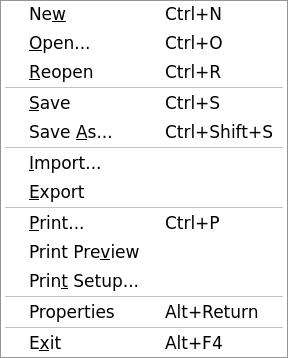
\includegraphics[width=\textwidth]{images/menu-File.png}\end{minipage}\hfill
\begin{minipage}[t]{0.58\textwidth}\vspace{0pt}
\begin{itemize}[leftmargin=1em]
  \item \menu{New}, \menu{Open\ldots}, \menu{Reopen} (loads the song from the last saved version), \menu{Save}, \menu{Save As\ldots}:
        the song is an \texttt{.rmt} file; \texttt{.txt} and \texttt{.rmw} are chosen in the file type of the dialog.
  \item \menu{Import\ldots}: ProTracker modules and TMC songs (chapter~\ref{ch:importexport}).
  \item \menu{Export}: the formats for the Atari (chapter~\ref{ch:importexport}).
  \item \menu{Print}, \menu{Print Preview}, \menu{Print Setup}: the screen of the song is printed on a landscape page, scaled to fill it.
  \item \menu{Properties} (\key{ALT+ENTER}): the properties of the song.
\end{itemize}
\end{minipage}

\section{Edit}

\begin{minipage}[t]{0.5\textwidth}\vspace{0pt}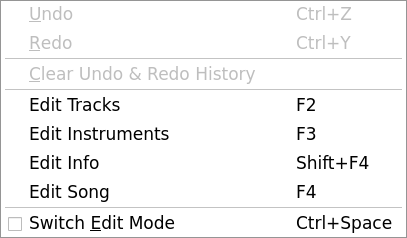
\includegraphics[width=\textwidth]{images/menu-Edit.png}\end{minipage}\hfill
\begin{minipage}[t]{0.46\textwidth}\vspace{0pt}
Undo and redo (the history can be cleared), the four parts of the screen (tracks, instruments, info, song), and the switch between
edit and prove mode.
\end{minipage}

\section{View}

\begin{minipage}[t]{0.36\textwidth}\vspace{0pt}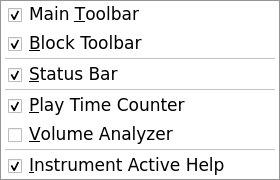
\includegraphics[width=\textwidth]{images/menu-View.png}\end{minipage}\hfill
\begin{minipage}[t]{0.6\textwidth}\vspace{0pt}
Shows or hides the toolbars and the status bar, the play time counter, the volume analyzer and the instrument active help. The
choices are kept in the configuration.
\end{minipage}

\section{Play}

\begin{minipage}[t]{0.5\textwidth}\vspace{0pt}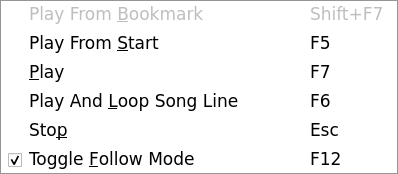
\includegraphics[width=\textwidth]{images/menu-Play.png}\end{minipage}\hfill
\begin{minipage}[t]{0.46\textwidth}\vspace{0pt}
Play from the bookmark, from the start, from the cursor, loop the song line, stop and follow mode (chapter~\ref{ch:playing}).
\end{minipage}

\section{Channels}

\begin{minipage}[t]{0.5\textwidth}\vspace{0pt}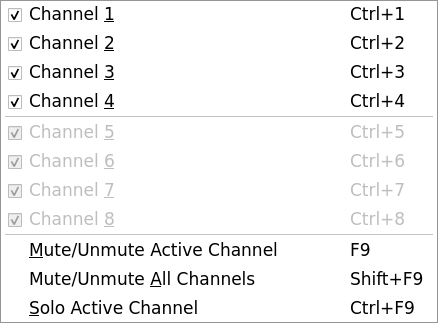
\includegraphics[width=\textwidth]{images/menu-Channels.png}\end{minipage}\hfill
\begin{minipage}[t]{0.46\textwidth}\vspace{0pt}
Switch on and off each of the channels 1 to 8, mute or unmute the active one or all of them, or play the active one alone.
\end{minipage}

\section{Song}

\begin{minipage}[t]{0.58\textwidth}\vspace{0pt}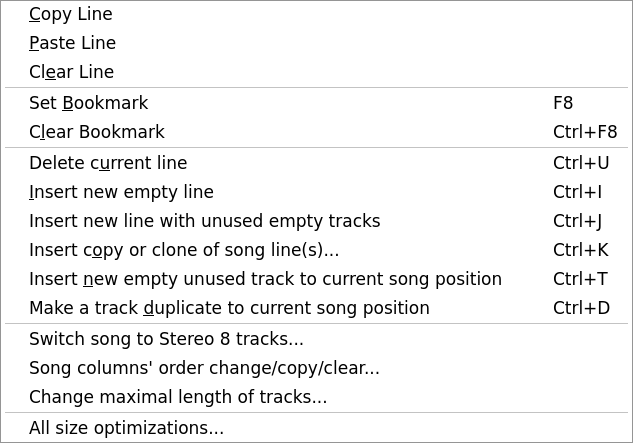
\includegraphics[width=\textwidth]{images/menu-Song.png}\end{minipage}\hfill
\begin{minipage}[t]{0.38\textwidth}\vspace{0pt}
Copy, paste and clear a song line; the bookmark; insert and delete lines; insert tracks; and the commands of chapter~\ref{ch:song}
that change the whole song.
\end{minipage}

\section{Instrument}

\begin{minipage}[t]{0.5\textwidth}\vspace{0pt}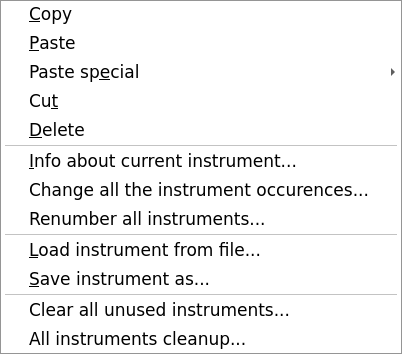
\includegraphics[width=\textwidth]{images/menu-Instrument.png}\end{minipage}\hfill
\begin{minipage}[t]{0.46\textwidth}\vspace{0pt}
Everything to do with an instrument: copy and paste (and paste special), information, change or renumber, clear the unused ones,
load and save (chapter~\ref{ch:instruments}).
\end{minipage}

\section{Track}

\begin{minipage}[t]{0.58\textwidth}\vspace{0pt}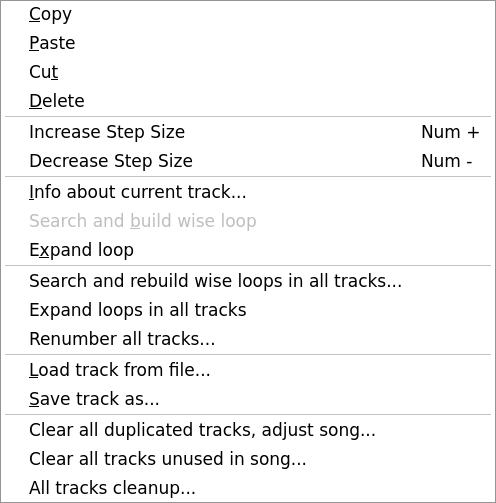
\includegraphics[width=\textwidth]{images/menu-Track.png}\end{minipage}\hfill
\begin{minipage}[t]{0.38\textwidth}\vspace{0pt}
Copy, paste, cut and delete a track; the step size; information about the current track; wise loops; renumbering; loading and saving a
track; and the clean-up of the tracks of the song.
\end{minipage}

\section{Block}

\begin{minipage}[t]{0.5\textwidth}\vspace{0pt}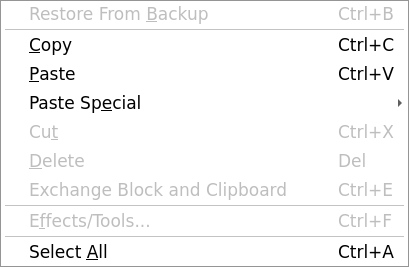
\includegraphics[width=\textwidth]{images/menu-Block.png}\end{minipage}\hfill
\begin{minipage}[t]{0.46\textwidth}\vspace{0pt}
The commands of the blocks (chapter~\ref{ch:tracks}): restore from the backup, copy, paste, paste special (merge, only the volumes, only the
speeds), cut, delete, exchange, effects and tools, select all.
\end{minipage}

\section{Pokey}

\begin{minipage}[t]{0.58\textwidth}\vspace{0pt}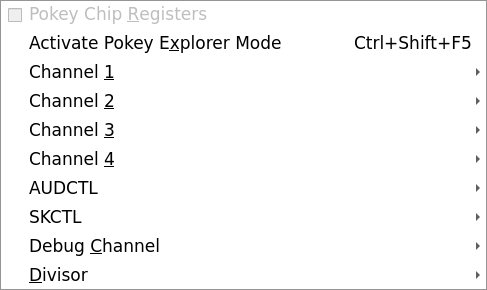
\includegraphics[width=\textwidth]{images/menu-Pokey.png}\end{minipage}\hfill
\begin{minipage}[t]{0.38\textwidth}\vspace{0pt}
The registers of the chip and the Pokey explorer mode, with a submenu for each channel (chapter~\ref{ch:explorer}).
\end{minipage}

\section{Tools}

\begin{minipage}[t]{0.35\textwidth}\vspace{0pt}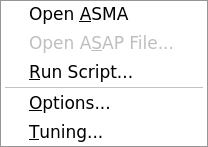
\includegraphics[width=\textwidth]{images/menu-Tools.png}\end{minipage}\hfill
\begin{minipage}[t]{0.61\textwidth}\vspace{0pt}
\menu{Open ASMA} opens the Atari SAP Music Archive in the browser; \menu{Run Script\ldots} runs a script
(chapter~\ref{ch:scripting}); \menu{Options\ldots} and \menu{Tuning\ldots} open the dialogs of chapter~\ref{ch:options}.
\end{minipage}

\section{Help}

\begin{minipage}[t]{0.32\textwidth}\vspace{0pt}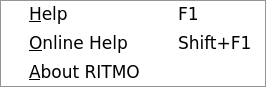
\includegraphics[width=\textwidth]{images/menu-Help.png}\end{minipage}\hfill
\begin{minipage}[t]{0.64\textwidth}\vspace{0pt}
The online help (a browser page with the documentation) and the \menu{About} window, with the credits.
\end{minipage}

\chapter{Options and tuning}\label{ch:options}

\section{The Options dialog}\label{sec:options}

\menu{Tools $\rightarrow$ Options\ldots} opens the dialog of figure~\ref{fig:dialog-options}. The settings are saved when the
program closes, in the settings of the system (chapter~\ref{ch:install}).

\dialog{dialog-options}{The \menu{Options} dialog.}{9.5cm}

\subsection{General}

\begin{description}[style=nextline,leftmargin=1.2cm]
  \item[Interface size (in \%)] The size of the drawing of the window, from 100\% to 300\%. Only whole multiples of 100\% keep
        the pixels exact.
  \item[Track line highlight step] The two numbers of the \texttt{HIGHLIGHT} field of the info area: every how many lines the lines of
        the tracks are highlighted (for example 8 and 4).
  \item[Use German notation] The note \texttt{B} is written \texttt{H}, as in the German notation.
  \item[Alternative track line numbering] The line numbers follow the highlight step.
  \item[Display accidentals as flats instead of sharps] \texttt{D\#} is written as \texttt{Eb}.
  \item[NTSC system speed (60 Hz)] The video system of the song: 60 frames a second instead of the 50 of PAL. The same switch is
        \key{CONTROL+F12}.
  \item[Don't use hardware soundbuffer] A different way of playing the sound buffer, for the audio systems that need it.
  \item[Smooth scroll during playback] The lines of the tracks scroll one pixel at a time while a song plays.
  \item[Debug display] A line of internal values in the status bar. Enable it only if you know what it shows.
  \item[RMT Driver Version] The tracker driver, the player routine that makes the sound while you work (chapter~\ref{ch:drivers}). The
        driver must be the one the song was made with; the default is \emph{RMT 1.34 Patch16 by VinsCool}.
\end{description}

\subsection{Keyboard}

\begin{description}[style=nextline,leftmargin=1.2cm]
  \item[Keyboard layout] QWERTY, QWERTZ or AZERTY: where the piano of the note keys is. The first start picks the layout from the
        language of the keyboard.
  \item[Move to previous/next song line while track boundaries are crossed] The cursor passes from the end of a track to the next
        song line, and the other way round.
  \item[Remember octaves and volumes separately for each instrument] Each instrument keeps the octave and the volume you last used with it.
  \item[Reset the Atari sound routines each time ESC is pressed] \key{ESC} also starts the player routine again.
  \item[Prompt a save dialog box each time CTRL+S is pressed] \key{CONTROL+S} asks where to save, also from the menu and the
        toolbar.
\end{description}

\subsection{MIDI}

The MIDI input device, the touch response, the Atari volume offset and \emph{Record note off}: they are described in
chapter~\ref{ch:midi}.

\subsection{Paths}

The \menu{Paths\ldots} button opens a dialog with the default folders of the songs, the instruments and the tracks, each with a
\menu{Browse} button. The dialogs to open and save start there.

\section{The tuning}

\menu{Tools $\rightarrow$ Tuning\ldots} (figure~\ref{fig:dialog-tuning}) is a calculator for the pitch of the notes. The POKEY makes its
frequencies by dividing a clock, so not every pitch exists: the program computes the divisors that come nearest to the notes of
the temperament you choose, and the tracker plays with them.

\dialog{dialog-tuning}{The \menu{Tuning} dialog.}{10cm}

\begin{description}[style=nextline,leftmargin=1.2cm]
  \item[Base tuning (Hz) and Base note] The frequency of a reference note, by default \texttt{A-} at 440.8375\ldots\,Hz. It can be any
        number: \texttt{432}, \texttt{443.9}\ldots
  \item[Temperament] \emph{Equal Temperament} (the default) or another. The \emph{Ratio} table lists the interval of each step over the unison
        as a fraction.
  \item[Reset] puts the default values back; \menu{Test now} tries the tuning.
\end{description}

The tuning is saved with the configuration and is also the one a script uses when it exports a song (chapter~\ref{ch:scripting}).

\chapter{Import and export}\label{ch:importexport}

\section{Importing}

\menu{File $\rightarrow$ Import\ldots} reads a ProTracker module (\texttt{.mod}) or a TMC song (\texttt{.tmc}, \texttt{.tm8}) and
makes a song of it. After the file is chosen the dialog of figure~\ref{fig:dialog-import} asks how to convert a module.

\dialog{dialog-import}{Importing a ProTracker module.}{11cm}

\begin{itemize}
  \item The \emph{type of RMT module}: \texttt{RMT4} (the four channels of the module on the four tracks) or \texttt{RMT8}
        (the channels spread on the two POKEYs, in the order 1, 4 / 2, 3).
  \item The treatment of the \emph{notes} (shift the octave down if the tuning of the song is too high, replace the portamento
        effects by calculated notes), of the \emph{volumes}, and the \emph{size optimizations} that are made while importing (wise loops, cutting
        the unused parts of the tracks).
\end{itemize}

When the conversion is done a dialog reports how many tracks, instruments and song lines the song has, and what the optimizations did.
Check the box and press \menu{OK}: the song is loaded, but it still needs your work. The instruments are rough: look at their envelopes and
distortions (drums, basses\ldots) and correct the tunings of the original samples.

\dialog{dialog-import-2}{The result of the import.}{9cm}

\section{Exporting}

\menu{File $\rightarrow$ Export} writes the song in a format for the Atari. The file dialog chooses the name and the format; most of the
formats then show a dialog of options. Every format is written from the data of the song as the tracker plays it.

\begin{center}
\begin{tabular}{@{}p{4.2cm}p{9.6cm}@{}}
\toprule
Format & Use \\ \midrule
RMT stripped song file (\texttt{.rmt}) & the module without the names and the unused tracks and instruments, to link in a program that uses
  the RMT player routine \\
ASM simple notation (\texttt{.asm}) & the notes as assembler data, for your own player \\
SAP-R data stream (\texttt{.sapr}) & the register writes of the POKEY, frame by frame \\
Compressed SAP-R (\texttt{.lzss}) & the same, compressed, for the LZSS player \\
SAP file + LZSS driver (\texttt{.sap}) & a file the Atari players (ASAP, the plug-ins of many players, ASMA) play directly \\
XEX Atari executable (\texttt{.xex}) & a program for the Atari that plays the song when it is started \\
Relocatable ASM for RMTPlayer (\texttt{.asm}) & the module as source with labels, to be placed in memory by your program \\
WAV audio file (\texttt{.wav}) & the sound as a 16-bit, 44.1\,kHz, stereo file, the song played once up to its loop \\
\bottomrule
\end{tabular}
\end{center}

\subsection{RMT stripped}

\dialog{dialog-export-stripped-rmt}{The export of an RMT stripped file.}{10cm}

The \emph{from address} is where the module will be in the memory of the Atari; the program shows the range it takes. The
options are \emph{SFX support} (keep the unused tracks and instruments, for sound effects played by the game),
\emph{GlobalVolumeFade} (a variable the program can use to fade the music) and \emph{No songline start} (the song always starts from
song line 0). The text box lists the \emph{RMT FEATures} the song uses: if a game uses only this song, these definitions can be pasted into
the player routine source (\texttt{rmt\_feat.a65}), which then assembles to a smaller and faster routine
(this is described in the file \texttt{optimization.txt} that comes with the program).

\subsection{ASM simple notation}

\dialog{dialog-export-simple-asm}{The export of the notes as assembler data.}{8cm}

Choose what to export (the tracks, or the whole song by song columns), how the note is written (the index \texttt{\$00}--\texttt{\$3C}, or the
frequency according to the distortion of the instrument), how the duration is written (notes only, with the special value
\texttt{XXX} in empty beats, or pairs of note and duration, in either order) and the prefix of the labels (empty for none).

\subsection{SAP, SAP-R and LZSS}

\dialog{dialog-export-sap}{The export of a SAP file.}{8cm}

A SAP file has a header with the name, the author and the date, which the dialog fills with those of the song. The field
\emph{Subsongs} lists, in hexadecimal, the song line each subsong starts from: \texttt{00} for one tune, \texttt{00 10} for two. SAP-R is the stream of
the POKEY registers; LZSS compresses it, and the SAP file contains it with the player routine of the VU-Player.

\subsection{XEX}

\dialog{dialog-export-xex}{The export of an Atari executable.}{10cm}

The program an XEX file contains shows a text on the Atari screen while it plays: up to five lines of 40 characters (the fifth shown
instead of the fourth when the \key{SHIFT} key of the Atari is held down). Below, the \emph{rasterbar} shows the CPU usage of the player
in colour, \emph{shuffle} changes its colours, and the box \emph{Automatically adjust playback speed}, with the line that says that the speed will be
adjusted to 50\,Hz on both PAL and NTSC systems, turns the adjustment of the speed on. The preview shows
the text as the Atari will draw it.

\subsection{Relocatable ASM}

\dialog{dialog-export-reloc-asm}{The export of a relocatable module.}{10cm}

The module is written as byte definitions with labels (the one of the start of the song data, and optionally separate labels for the
instruments, the tracks and the song lines, which can be placed in different places of memory). The text box shows the size of each
part and the order of the modules.

\subsection{WAV}

The WAV export has no options: it plays the song with the built-in emulation and writes the sound.

\section{Exporting from the command line}

All the formats can be exported from a script, with no window, so that the files of a release are made from the \texttt{.rmt}
source (chapter~\ref{ch:scripting}).

\chapter{MIDI input}\label{ch:midi}

\RITMO{} plays and records notes from a MIDI keyboard. The input device is chosen in \menu{Tools $\rightarrow$ Options} (the MIDI
group); the button \menu{Toggle MIDI on/off} of the toolbar switches the input on and off while a device is set. The device is a port
of the system: on Linux the ports of the ALSA sequencer (a USB keyboard or a virtual port), on Windows WinMM, on macOS CoreMIDI.

\section{Options}

\begin{center}
\begin{tabular}{@{}lp{10.2cm}@{}}
\toprule
Option & Meaning \\ \midrule
MIDI IN device & the input device, or \emph{none} \\
Touch response & the key velocity becomes the volume of the note: \texttt{Atari Volume Offset + velocity / 8}, limited to 1--15. Without it the
  current volume (as for the typed notes) is used \\
Atari volume offset & added to the volume of the velocity, from 0 to 15 \\
Record note off & a released key (a note off, or a note on with velocity 0) deletes the note it played and writes volume 0. Without it releases are
  ignored \\
\bottomrule
\end{tabular}
\end{center}

\section{The MIDI channels}

\begin{center}
\begin{tabular}{@{}lp{10.5cm}@{}}
\toprule
Channel & Function \\ \midrule
1 & Records notes at the cursor, like the note keys: the MIDI note 36 is the lowest note of the tracker (\texttt{C-1}), the note is written with the
  active instrument, the cursor moves down by the note spacing, and the note is played. While the song plays with follow mode, a note in the
  first half of a line is written on the next line (quantized). Outside the tracks area, in a jam mode or with \key{SHIFT} or \key{CONTROL} held down, the note is only
  played. Recording needs the window to have the focus \\
2--9 & Live play on the channels \texttt{L1}--\texttt{L4} and \texttt{R1}--\texttt{R4} (6--9 repeat \texttt{L1}--\texttt{L4} on a mono song): never
  recorded, and independent of the focus. The velocity is the volume (velocity / 8); a program change sets the instrument of the channel;
  the controller 123 (all notes off) stops its note and the controller 121 (reset all controllers) restarts the player routine \\
11--15 & a program change chooses the active instrument \\
10 and 16 & an experimental assignment of controllers, kept from the original program, with the \texttt{POKEY explorer} (chapter~\ref{ch:explorer}) on
  channel 16 \\
\bottomrule
\end{tabular}
\end{center}

A system reset message (\texttt{FF}) restarts the player routine and forgets the notes held on the channels 2 to 16. The implementation chart of
the MIDI messages is in appendix~\ref{app:midi}.

\section{Scripts}

A script can send MIDI messages to the program with the \texttt{midi} command, which is how the recording can be tested without a keyboard
(chapter~\ref{ch:scripting}).

\chapter{The Pokey explorer}\label{ch:explorer}

The explorer is a mode to study the sound of the POKEY. \menu{Pokey $\rightarrow$ Activate Pokey Explorer Mode}
(\key{CONTROL+SHIFT+F5}) stops the tracker's player routine and lets the keys write the registers of the chip directly, so that you can hear
the effect of each divisor, distortion and \texttt{AUDCTL} bit. The mode is left with the edit/jam toggle (\key{CONTROL+SPACE}).

\shot{window-explorer}{The Pokey explorer mode, with the registers of the chip on the screen.}{0.98}

With \menu{View $\rightarrow$ Pokey Chip Registers} on, three rows under the dumps of the registers detail one channel: its \texttt{AUDF} and
\texttt{AUDC} bytes, the first divisor of \texttt{AUDF + MODOFFSET} from 3 up (\texttt{MODULO}), the coarse divisor of the pitch formula (28 at
64\,kHz, 114 at 15\,kHz, 1 at 1.79\,MHz and for joined channels), the free divisor, the modulo offset (1, 4 at 1.79\,MHz, 7 for joined channels)
and the resulting pitch.

\section{The keys}

The keys are the physical positions of the QWERTY layout (on QWERTZ and AZERTY they are the keys at the same positions).

\begin{center}
\begin{tabular}{@{}lp{10.5cm}@{}}
\toprule
Key & Function \\ \midrule
\key{ENTER} / \key{BACKSPACE} & next / previous channel (0--3) \\
\key{+} / \key{-} & divisor $+0.1$ / $-0.1$; with \key{SHIFT} $+1.0$ / $-1.0$ (from 1.0 to 10000.0) \\
\key{1} \key{3} \key{5} \key{7} & \texttt{AUDF0} to \texttt{AUDF3} $+1$; with \key{SHIFT} $+\$10$ \\
\key{Q} \key{E} \key{T} \key{U} & \texttt{AUDF0} to \texttt{AUDF3} $-1$; with \key{SHIFT} $-\$10$ \\
\key{2} \key{4} \key{6} \key{8} & \texttt{AUDC0} to \texttt{AUDC3} $+1$; with \key{SHIFT} $+\$10$ \\
\key{W} \key{R} \key{Y} \key{I} & \texttt{AUDC0} to \texttt{AUDC3} $-1$; with \key{SHIFT} $-\$10$ \\
\key{C} \key{G} \key{F} \key{K} \key{J} \key{D} \key{A} \key{P} & toggle the bits 0 to 7 of \texttt{AUDCTL}: the 15\,kHz clock, the two high pass filters, the
  two 16-bit joins, the two 1.79\,MHz clocks and the 9-bit poly counter \\
\key{M} & toggle the two-tone bits of \texttt{SKCTL} \\
\bottomrule
\end{tabular}
\end{center}

The \menu{Pokey} menu has the same operations as menu items, which work in the explorer mode only.

\chapter{Tracker drivers}\label{ch:drivers}

\input{generated/drivers.tex}

\chapter{Scripting}\label{ch:scripting}

\input{generated/scripting.tex}


\appendix
\chapter{Reference of the commands, keys and fields}\label{app:reference}

This appendix is the complete reference: every command of the menus and the toolbars with its key, the note keys of the three keyboard
layouts, and the keys and the fields of each part of the screen. The first two tables are written by the program itself.

\input{generated/reference.tex}

\chapter{The RMT module file format}\label{app:format}

The format of the \texttt{.rmt} files, for the programmers who read them. It is the format version~1, used by all the RMT trackers up to
now; the description is the official one of the repository.

\input{generated/format.tex}

\chapter{MIDI implementation chart}\label{app:midi}

The MIDI implementation chart of the multitimbral instrument that the tracker is, from the original documentation of \RMT{} (the
program also accepts the controllers described in chapter~\ref{ch:midi}).

{\scriptsize
\lstinputlisting[basicstyle=\ttfamily\scriptsize,frame=none,backgroundcolor=\color{white},breaklines=false]{generated/midi.txt}
}

\chapter{Building from the source}\label{app:building}

\RITMO{} is built with CMake and Qt. The full instructions are in the file \texttt{BUILD.md} of the source; here is the short version.

\section{Linux}

\begin{lstlisting}
sudo apt install cmake qt6-base-dev portaudio19-dev librtmidi-dev
cmake -B build-qt -DCMAKE_BUILD_TYPE=Release
cmake --build build-qt -j
./build-qt/out/ritmo song.rmt
\end{lstlisting}

The program is \texttt{build-qt/out/ritmo}, with the \texttt{resources} folder next to it. \texttt{-DRMT\_QT\_MAJOR=5} builds with
Qt~5.15 instead of Qt~6.

\section{Windows and macOS}

Windows is built with MSYS2 (MinGW64: GCC, Qt~6, PortAudio, RtMidi) and macOS with the Apple compiler and the Qt of the official installer. The
GitHub workflows of the repository (\texttt{.github/workflows}) build the packages of both, and the AppImage for Linux
(\texttt{scripts/build-appimage.sh}), and are the best description of the steps.

\section{Core only and tests}

\texttt{-DRMT\_BUILD\_CORE\_ONLY=ON} builds the engine and the audio and MIDI backends without Qt, and with \texttt{-DRMT\_CORE\_TEST=ON}
the \texttt{RmtCoreTest} program, a smoke test of the engine. The \texttt{scripts/test-scripting.sh} script runs the reference scripts.

\section{Test hooks}

For tests and documentation the program can run without a display (\texttt{QT\_QPA\_PLATFORM=offscreen}). The environment variables
\texttt{RMT\_QT\_GRAB} (save the window and quit), \texttt{RMT\_QT\_KEYS}, \texttt{RMT\_QT\_COMMANDS}, \texttt{RMT\_QT\_FILEDIALOG},
\texttt{RMT\_QT\_DIALOG} and \texttt{RMT\_QT\_MENU\_GRAB} (the menus as images) press keys, run menu commands, answer the dialogs and save them. The
screenshots of this manual were taken that way, by \texttt{doc/manual/make-screenshots.sh}.

\chapter{Credits and licenses}\label{app:credits}

\section{Credits}

\begin{itemize}
  \item Radek \v{S}t\v{e}rba, Raster/C.P.U., 2002--2009 (R.I.P.). The original RASTER Music Tracker. Thank you for everything you did; we truly miss you.
  \item Robert Petruzela (Bob!k/C.P.U.) and JirkaS/C.P.U.
  \item Vin Samuel (VinsCool), 2021--2024: RMT 1.31 to 1.34, the POKEY tuning calculations, the SAP-R dumper and the VU-Player, and much more.
  \item Peter Dell (JAC!), 2024 to present: RMT 1.35 and the base of this fork.
  \item Gianluca Renzi, 2026: the Qt port and the RITMO fork (Linux, Windows, macOS).
\end{itemize}

Also: the LZSS compression is by DMSC, ported to C++ by VinsCool; the unrolled LZSS music driver is by Rensoupp; the bitmap graphics, the ideas and the
beta testing are by PG; advice on tuning from synthpopalooza and OPNA2608; ideas and suggestions from Enderdude, Spring, Ivop, Tatqoo and Miker.
Thanks to Fox/Taquart (XASM and ASAP), Jaskier/Taquart (TMC and optimizations of the RMT routines), the people of the Chiptune Caf\'e, AtariAge and
GBAtemp, the Polish Atarians of Atariarea and all the 8-bit Atarians of the world.

\section{The fonts}

The logo and the icon of \RITMO{}, and the cover of this manual, are drawn with the glyphs of the IBM VGA 9x16 font, in the version \emph{PxPlus IBM VGA 9x16} of
\emph{The Ultimate Oldschool PC Font Pack} by VileR (\url{https://int10h.org/oldschool-pc-fonts/}), licensed under CC BY-SA 4.0.

\section{Disclaimer}

\RMT{} IS A SOFTWARE WITHOUT WARRANTY OF ANY KIND. THE AUTHOR DOES NOT WARRANT, GUARANTEE, OR MAKE ANY REPRESENTATIONS REGARDING THE USE, OR THE RESULTS OF
USE OF THE SOFTWARE, OR WRITTEN MATERIALS, IN TERMS OF CORRECTNESS, ACCURACY, RELIABILITY, CURRENTNESS, OR OTHERWISE. THE ENTIRE RISK AS TO THE RESULTS
AND PERFORMANCE OF THE SOFTWARE IS ASSUMED BY YOU.


\end{document}
